\section{Usage}
The GeoLog was designed for the field scientist or any one how is interested in monitoring the enviroment. The GeoLog was designed for rough enviroment, thus it can be left out side in rugged terrain.\\
The knowledge one needs for building and maintain his own Geo Log is a background in software C, C++ and some knowledge in electric circuits. % %For further development one would...

\subsection{Installation}
To prepare the system for use the first one would need to set up the necessary software to be able to configure the sampling rate of the desired data. The user needs to able to modify the Arduino sketch but should not be required to modify the Wixel software. Thus set up of the Arduino development enviroment is needed but for the Wixel it is optional.\\
All the required code for this system can be found under~\url{https://projects.cs.ru.is/projects/T-411-MECH/student/2014/group/DataCollector}, contact Joe Foley for gaining access. The link~\url{https://projects.cs.ru.is/projects/T-411-MECH/student/2014/group/DataCollector} will be referred as DataCollector-folder from here on.\\

\begin{enumerate}
\item Install the software
	\begin{enumerate}
	\item For the Arduino:
		\begin{enumerate}
		\item Start a web browser
		\item Goto~\url{http://arduino.cc/en/main/software}
		\item Install the appropriate version of Arduino IDE for your platform.
		\end{enumerate}
	\item For the Wixel:
		\begin{enumerate}
		\item Start a web browser
		\item Goto~\url{http://www.pololu.com/docs/0J46}
		\item Install the Wixel IDE
		\item Follow the instructions listed in part 10.a, 10.b and 10.c, for setting up the development enviroment
		\end{enumerate}
	\end{enumerate}
\item Set up the hardware
	\begin{enumerate}
	\item Connect the components for the mother hub.
		\begin{enumerate}
		\item Follow the diagram in \fxfatal{fix figure}figure~\ref{fig:??}
		\item Position the mother hub in its box as in figure~\ref{fig:Main_Open}
		\end{enumerate}
	\item Connect the components for the wireless sensor module/modules
		\begin{enumerate}
		\item Follow the diagram in \fxfatal{fix figure}figure~\ref{fig:??}
		\item Position the components in its box as in figure~\ref{fig:Wixel_sensor}
		\end{enumerate}
	\end{enumerate}
\item Upload the code
	\begin{enumerate}
	\item For the mother hub
		\begin{enumerate}
		\item On the Wixel..... % TODO: finish this list
		\item ....
		\end{enumerate}
	\end{enumerate} 
\end{enumerate}
% TODO: remember to mention the batteries
% TODO: set the sampling time and data transmission time

\begin{figure}[H]
\centering
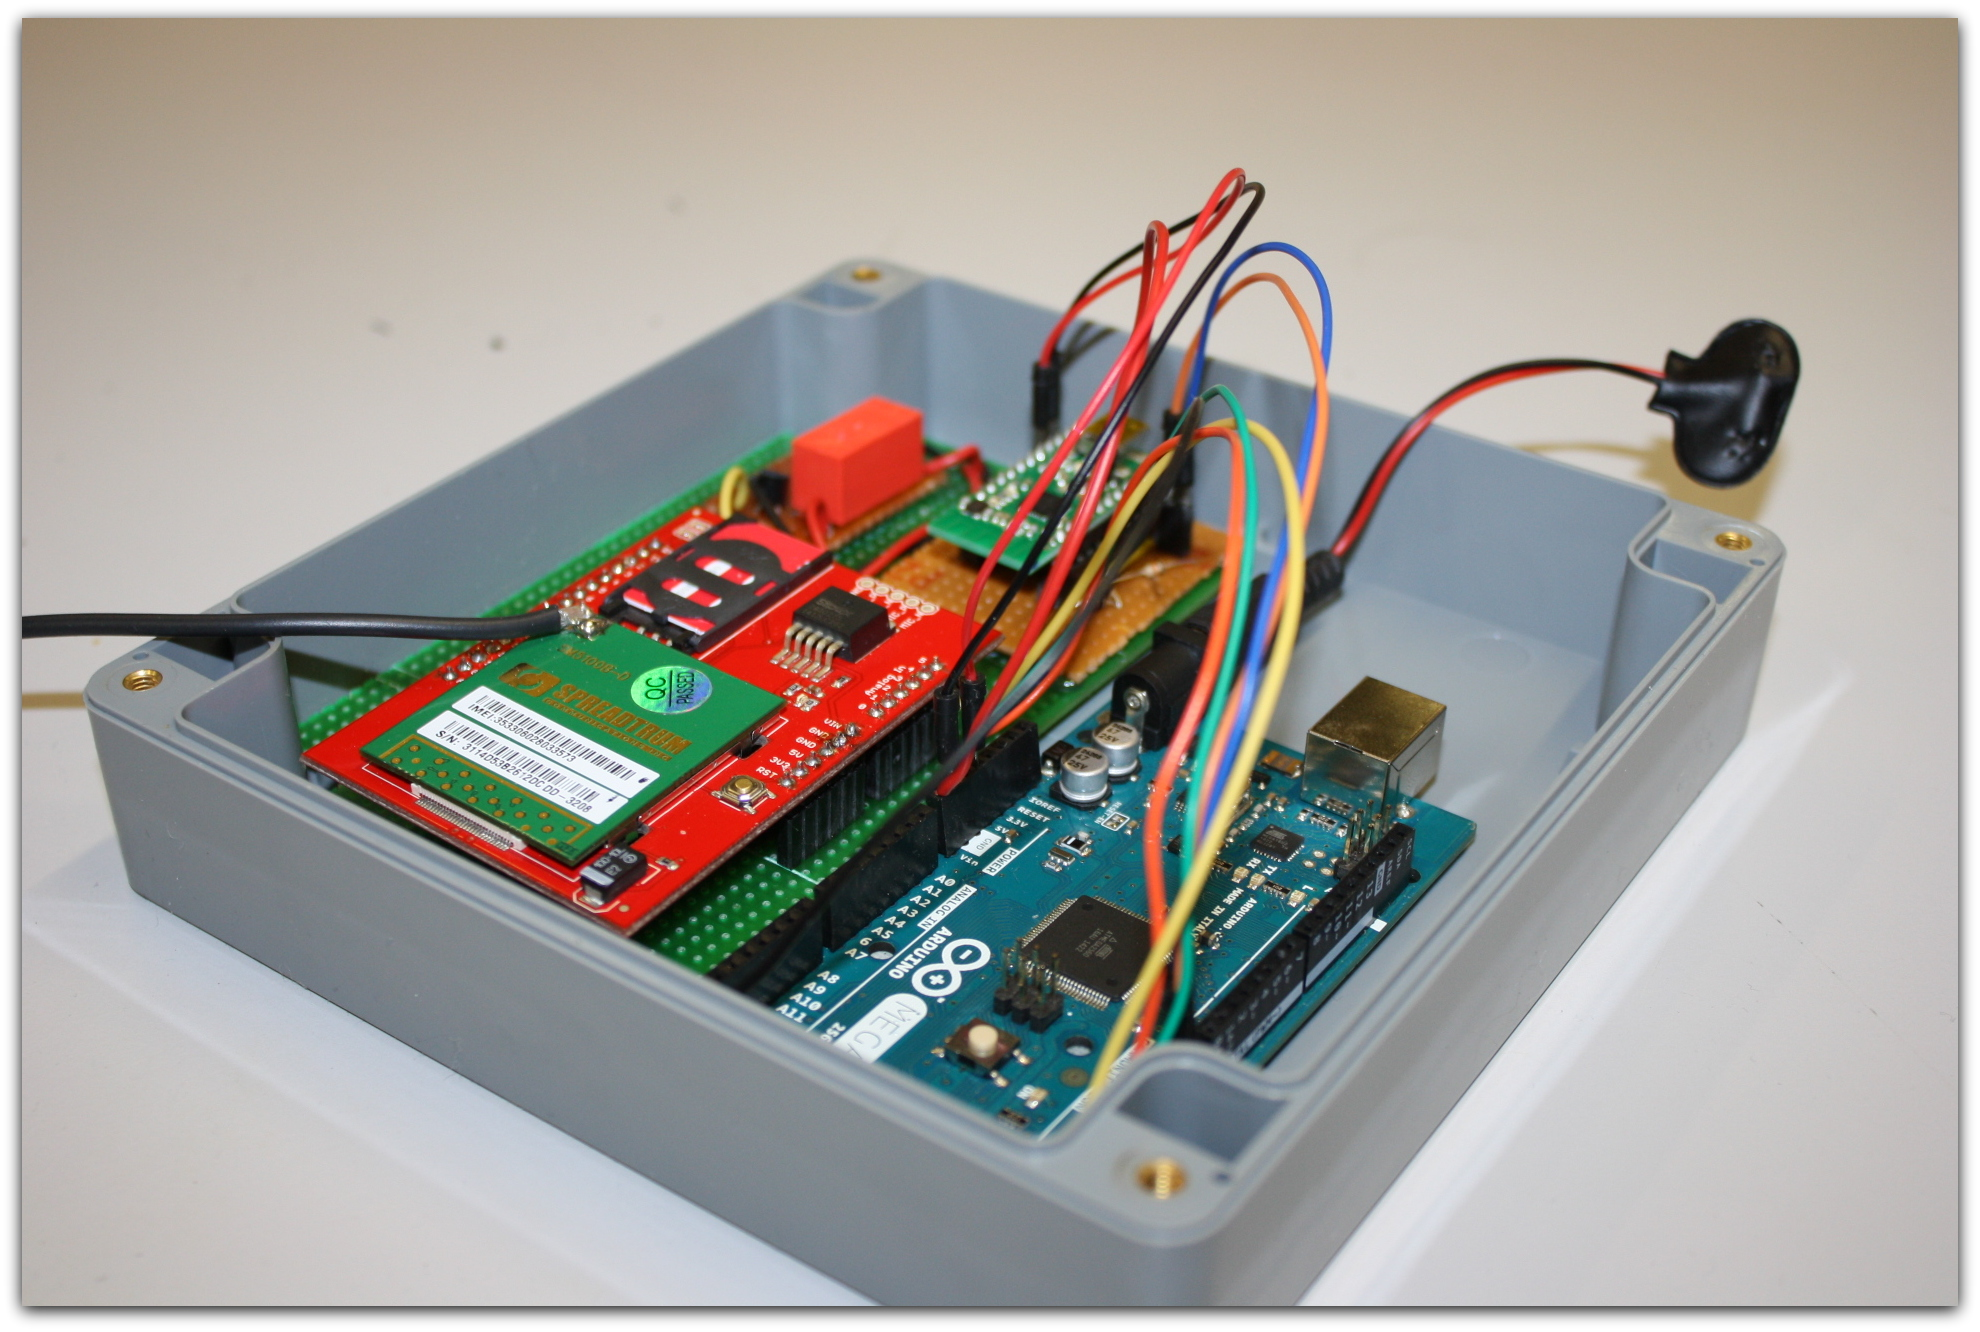
\includegraphics[width=0.6\linewidth]{graphics/Main_Open.jpg}
\caption{The mother hub displayed in its box\label{fig:Main_Open}}
\end{figure}
\begin{figure}[H]
\centering
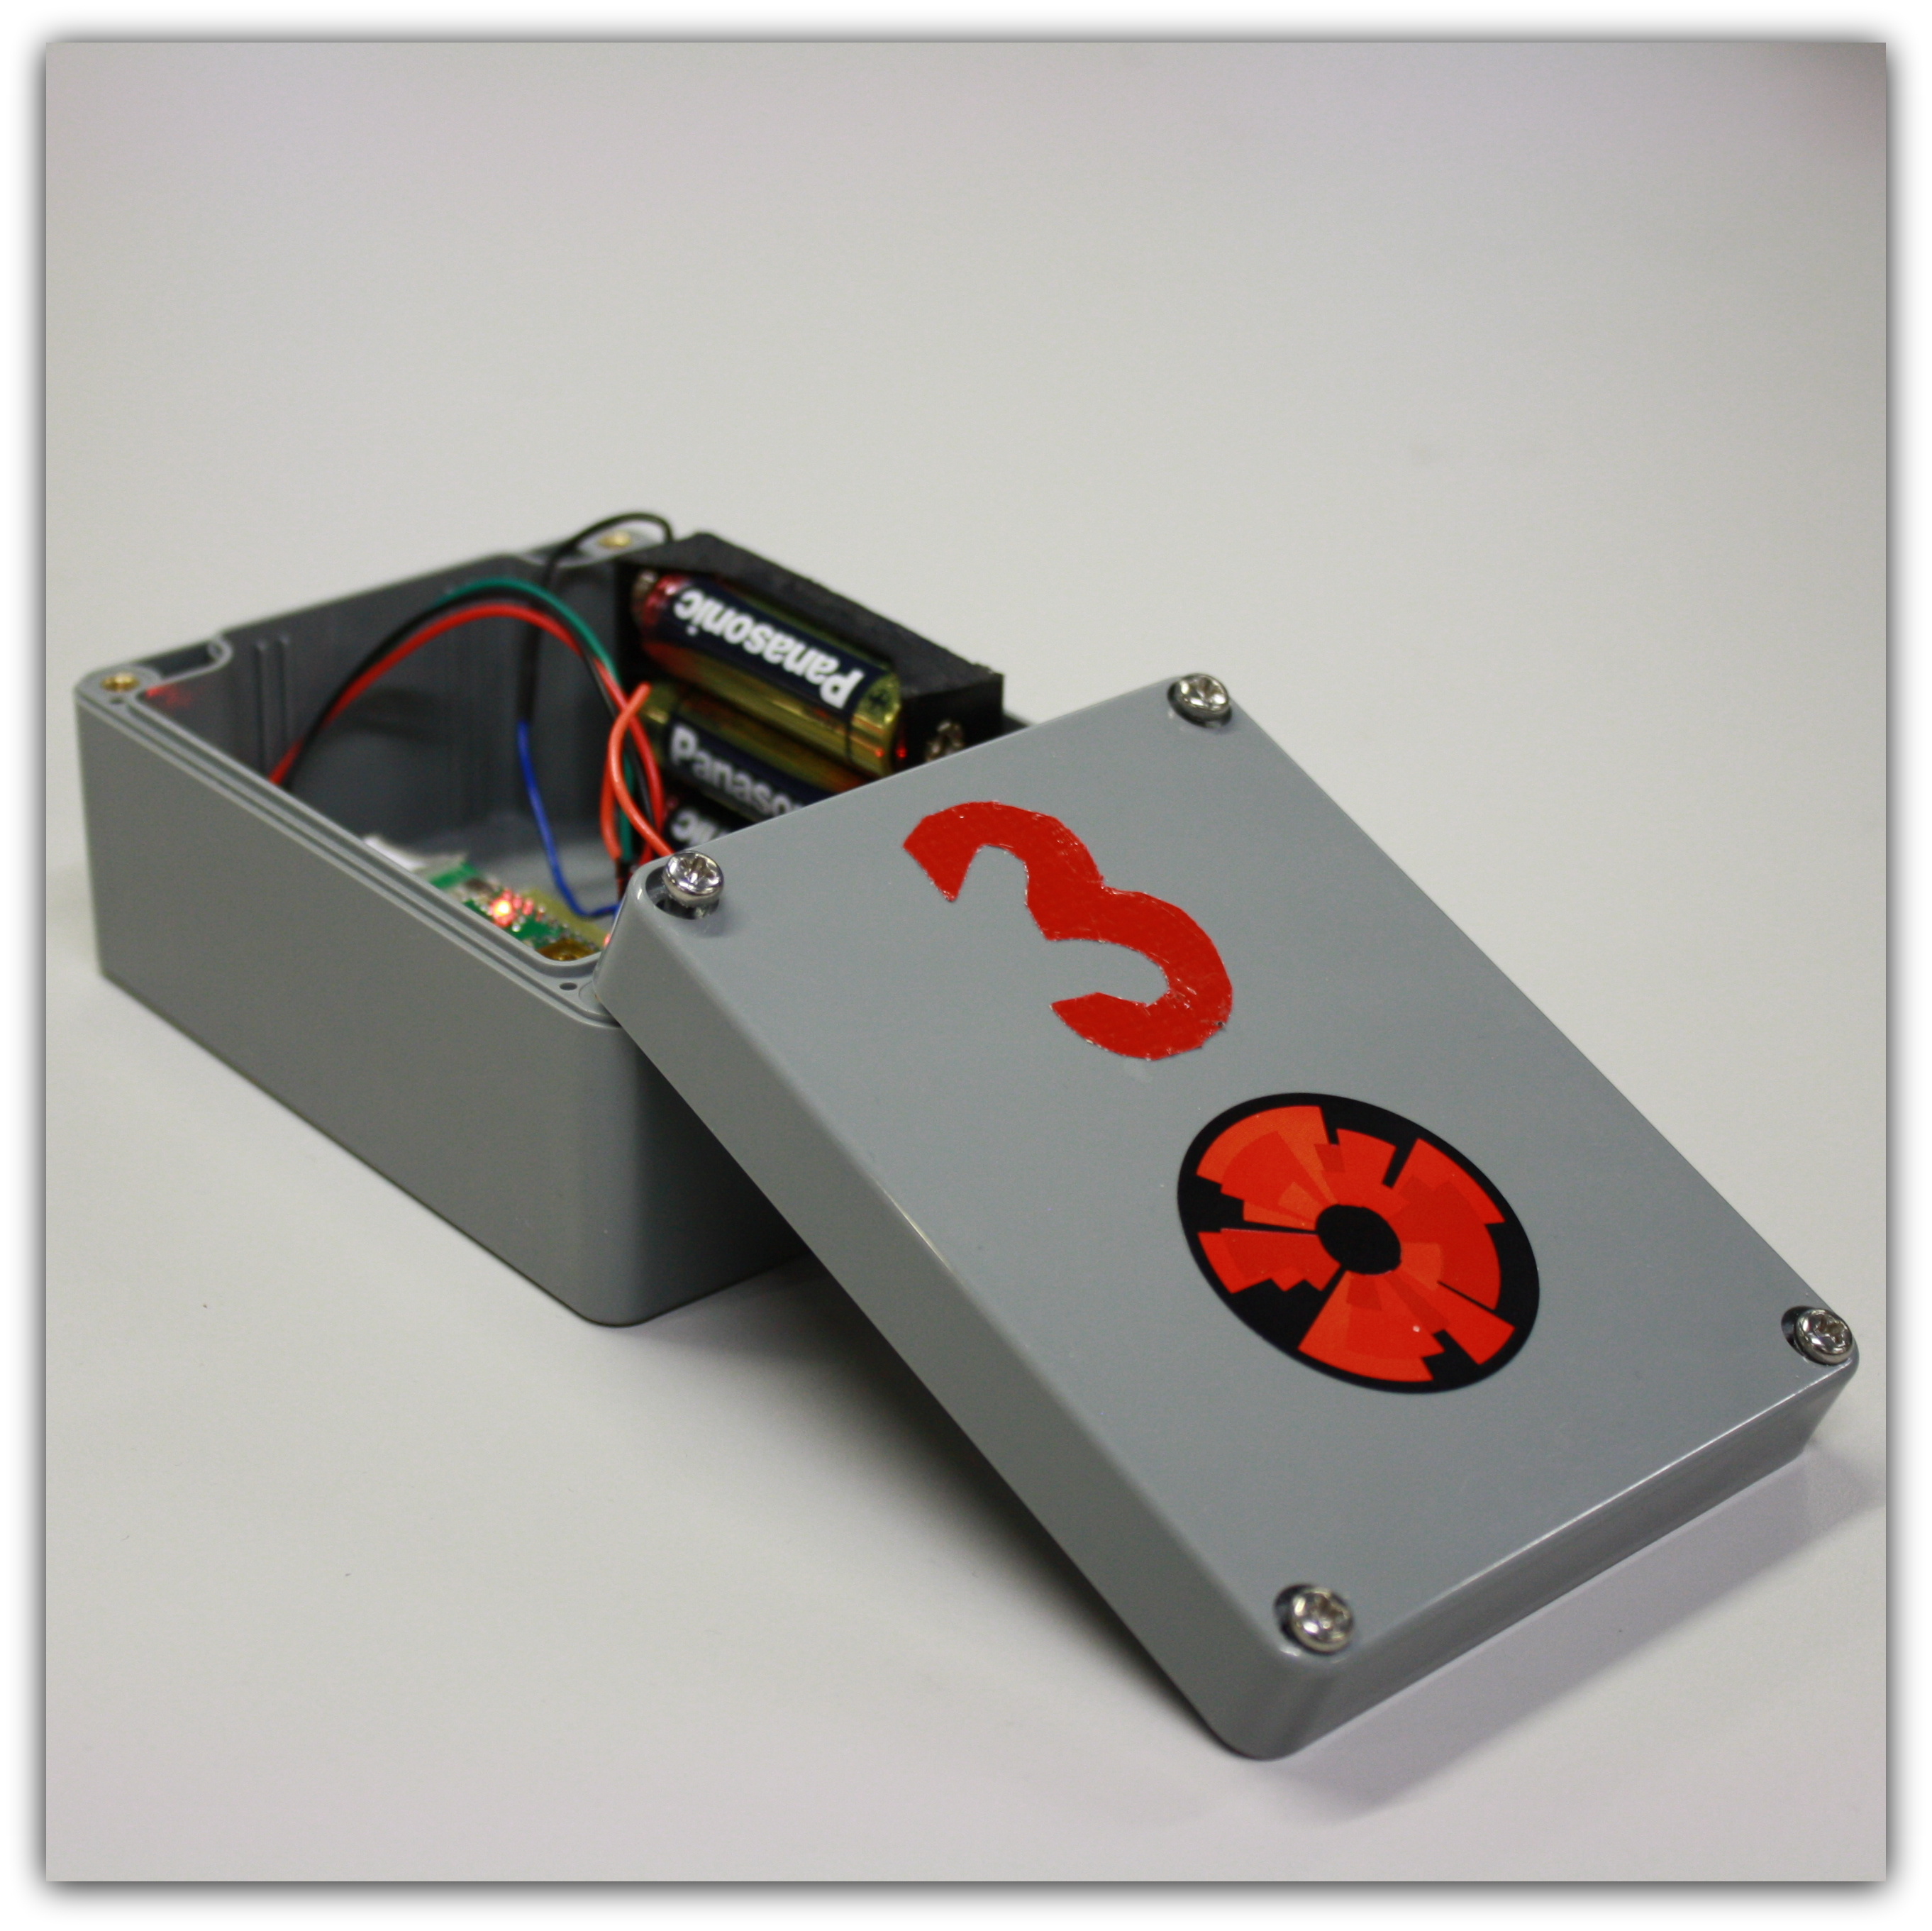
\includegraphics[width=0.6\linewidth]{graphics/Wixel_sensor.jpg}
\caption{The wireless sensor module in its box\label{fig:Wixel_sensor}}
\end{figure}

To prep the GeoLog for transport the batteries need to be removed out of the box for each module. The boxes should be securely closed with the four screws in each corner. Then the GeoLog is ready for travel.\\
To unpack the GeoLog open the boxes, insert the batteries and close the boxes again.

\subsection{Instructions}
Once the system is setup the user should be able to position the GeoLog in the site where data is to be collected. Spread out the wireless sensor module around the mother hub.\\
\textbf{Warning: the Wixel sensor module can not be placed more than 15m away from the mother hub}.\\
Set the sampling frequency and the data transmission time for the GeoLog to the desired values. To set the values the MainRunner.ino sketch that runs on the Arduino needs to be modified. The sketch can be found under DataCollector-folder/Software. Change the defined constants SAMPLE\_DATA\_FREQ and SEND\_DATA\_FREQ in line 13 and 14, the values for the sampling time should be given in milliseconds.\\






